\documentclass{article}

% if you need to pass options to natbib, use, e.g.:
%     \PassOptionsToPackage{numbers, compress}{natbib}
% before loading neurips_2021

% ready for submission
\usepackage[preprint]{common/neurips_2021}

% to compile a preprint version, e.g., for submission to arXiv, add add the
% [preprint] option:
%     \usepackage[preprint]{neurips_2021}

% to compile a camera-ready version, add the [final] option, e.g.:
%     \usepackage[final]{neurips_2021}

% to avoid loading the natbib package, add option nonatbib:
%    \usepackage[nonatbib]{neurips_2021}

\usepackage[utf8]{inputenc} % allow utf-8 input
\usepackage[T1]{fontenc}    % use 8-bit T1 fonts
\usepackage[colorlinks=true]{hyperref}       % hyperlinks
\usepackage{url}            % simple URL typesetting
\usepackage{booktabs}       % professional-quality tables
\usepackage{amsfonts}       % blackboard math symbols
\usepackage{nicefrac}       % compact symbols for 1/2, etc.
\usepackage{microtype}      % microtypography
\usepackage{xcolor}         % colors
\usepackage{amsmath}
\usepackage{graphicx}
\usepackage[]{placeins}

\setlength{\parindent}{0pt}

\title{Rotten Tomatoes Review Discrepancy}
\author{%
  Benjamin Raible\\
  Matrikelnummer 6413200\\
  \texttt{b.raible@student.uni-tuebingen.de} \\
  \And
  Daniel Kerezsy\\
  Matrikelnummer 6300575\\
  \texttt{daniel.kerezsy@student.uni-tuebingen.de} \\
  \And
  Andreas Kotzur\\
  Matrikelnummer 6479284\\
  \texttt{andreas.kotzur@student.uni-tuebingen.de} \\
}

\begin{document}
\maketitle
\begin{abstract}
    This project investigates the discrepancies between official critics' and the audience's ratings for movies on Rotten Tomatoes. We want to find out if there are any regularities and if these are enough to predict the scores (or their discrepancy/divergence). This project covers the data gathering and the evaluation with Null-Hypothesis Tests, Linear Regression, Decision Trees and MLPs. Results show that there is not enough information to infer any significant results.
\end{abstract}

\section{Introduction}
    There are a lot of websites rating the quality/perception of movies and TV series. One of the most popular ones is the US-American website \href{https://www.rottentomatoes.com}{https://www.rottentomatoes.com} \cite{rotten_about} which allows officially registered critics and the general audience to rate a movie resulting in a score between 0\% and 100\% for both voter categories. It is a relatively well known phenomenon that the opinions of these two parties often diverge and sometimes even by a huge amount. This observation can be made every so often and has thus obviously led to many discussions \cite{looper_divides}\cite{reddit_divide_1}\cite{reddit_divide_2}.\\
    We want to know if there are any commonalities between the movies where ratings diverge and thus need a database where all this information is combined.  
    We gather information about movies from the 1950s up to 2022 using Wikipedia lists and Rotten Tomatoes. We did not use \href{https://www.imdb.com/}{IMDb} since for us relevant data like the 'budget' or the 'box office' is hidden behind a paywall (IMDb Pro).

\section{Creating the Database}
    Since we could not find a compact and accessible database containing the data we need, the first logical step was to create our own. This requires gathering data at first, repairing as much as possible and finally filtering unusable or wrong entries.\\
    We use Python 3.10, Scrapy and Pandas for this process.

\subsection{Collecting the data}
% Benno plz correct me on this one
    We start by initially crawling through Wikipedia collecting URLs to entries of a specific movie and their corresponding year of release. These movies are listed under sublists, containing all movies worldwide released in that year. Note that the year under which the movie is listed does not necessarily represent the actual time of release.\\
    In a second crawler, this URL will then be used to gather information such as the name of the movie and the further more detailed information. \\
    These Wikipedia entries won't contain a link to their corresponding entry on Rotten Tomatoes. To acquire this entry without needing several steps (search, compare, filter) to eventually get to the corresponding entry, we used an heuristic approach.\\
    We found out that Rotten Tomatoes filters their URL entries before redirecting to the appropriate URL and resource. Using this information, we took the name of the movie, we could simply append the name of the movie to the URL.
    This works pretty well but is susceptible to remakes or different movies with the same name, e.g. Batman (1943), Batman (1966) and Batman (1989)\cite{batman_remakes}.
    Again we use heuristics to acquire the correct entry by simply appending the year to the query as in \texttt{"$<$movie\_name$>$\_$<$yyyy$>$"}. If we get a result we use it for our entry, otherwise we try querying the film without this appendix.
    Both data entries from Rotten Tomatoes (if any) and Wikipedia are then combined in our unrefined database. This way we acquired 19366 entries. %\\
    % The process of the data collection is also visualized in this Activity Diagram(\ref{fig:data_col_flow}).
    % % Might have to be deleted since it takes up too much space
    % \begin{figure}[tb]
    %     \centering
    %     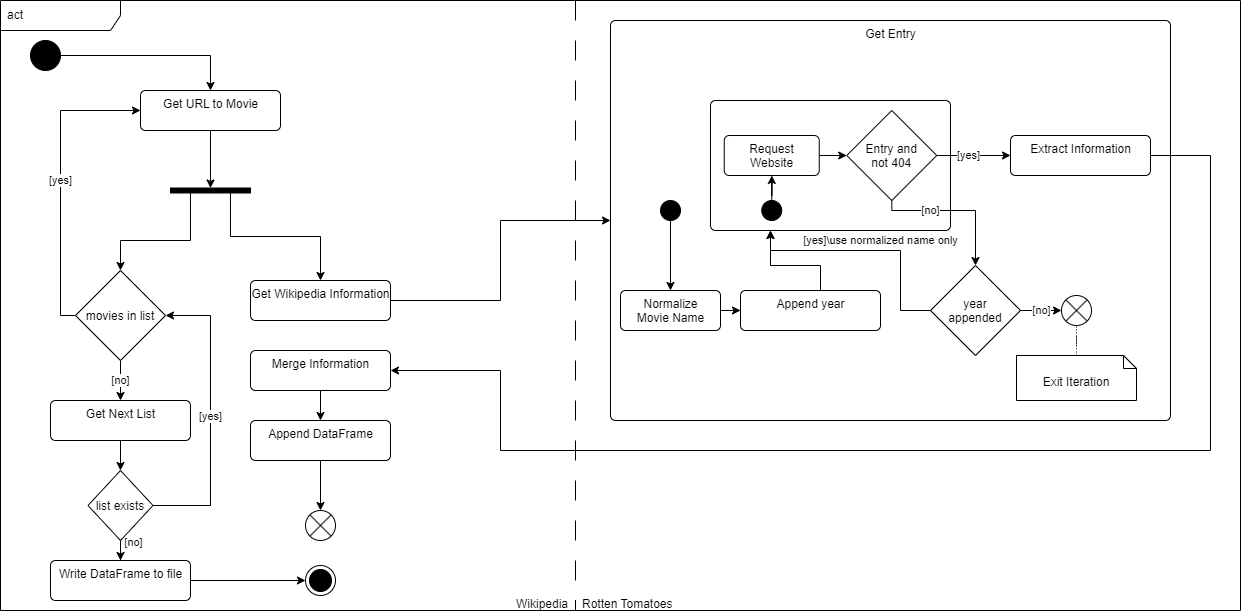
\includegraphics[width=1\textwidth]{imgs/activity_diagram.png}
    %     \caption{Data Collection Activity Diagram}
    %     \label{fig:data_col_flow}
    % \end{figure}

\subsection{Cleaning the data}
    In order to verify/clean our data from the applied heuristic, we extracted the release date gathered from Wikipedia and compared it with the date gathered from Rotten Tomatoes. We assume that a movie with the same name would not be released in the same year and thus removed all entries where the two different dates diverged resulting in a loss of 222 entries. \\
    One of our main goals for the data extraction was to gather information about the Box office (revenue) and the budget. Since our list contains movies from all around the world beginning from the 1950s, we have a lot of different currencies subjected to different inflation rates within our database. Furthermore, some of the Wikipedia entries already contain the converted currencies inclusive the inflation rate. In order to have a common ground, we convert all entries to US-Dollar with the inflation being accounted up to December 2022. We consider 15 different currencies, the release date and the potentially already converted values plus their corresponding date.\\
    To calculate the inflation rate we use the average Consumer Price Index (CPI) for all items obtained from a database by the \href{https://data.imf.org/?sk=388dfa60-1d26-4ade-b505-a05a558d9a42}{International Monetary Fond (IMF)}. Using a \href{https://www.kaggle.com/datasets/thebasss/currency-exchange-rates}{dataset containing 52 different currencies} which is also based on IMF data, we can convert all currencies into US-Dollar.

    % Needed for next section
    % \begin{figure}[h]
    %     \centering
    %     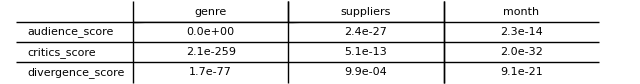
\includegraphics[width=1\textwidth]{imgs/var_p.png}
    %     \caption{FIXME}
    %     \label{fig:variance_p}
    % \end{figure}

% \clearpage
\section{Processing the data}
    % Nur gruppen mit >=100 occurences für genres und suppliers.
    % Critics Mean: 61.916190970420345, Deviation: 27.822854062556722
    % Audience Mean: 60.35768595041322, Deviation: 21.49258710416916
    % Divergence Mean: 0.9719551988711527, Deviation: 21.060031368055885
    
    % \begin{table}[h]
    %     \centering
    %     \begin{tabular}{c||c|c}
    %          & Mean & Std. Deviation \\ \hline
    %         Critics Score & 61.92 & 27.82 \\ \hline
    %         Audience Score & 60.36 & 21.49 \\ \hline
    %         Divergence & 0.97 & 21.06 
    %     \end{tabular}
    %     \caption{Mean and Standard Deviation of our targets}
    %     \label{tab:mean_std_target}
    % \end{table}

\subsection{Hypothesis tests}
    First we decided to perform hypothesis tests to see, if our parameters influence our targets. Audience and critics score on rotten tomatoes measure the percentage of people who submitted a positive review. It makes sense to measure the distance between this scores. This extends to their discrepancy. Therefore our target is metric. This now allows us to find the correct hypothesis tests.
    \paragraph{Parameters with multiple groups}
    For parameters that divide the data into multiple groups the corresponding hypothesis test is a simple analysis of variance combined with a post hoc test. In our case such parameters are the genre, streaming supplier and the release month.\\
    For our simple analysis of variance the two hypothesises are as follows:
    \begin{enumerate}
        \item[H0:] The mean scores of all groups are equal.
        \item[H1:] At least one of the mean scores of the groups differs.
    \end{enumerate}
    We set our significance level to 0.05.\\
    \noindent
    \begin{figure}[h]
        \centering
        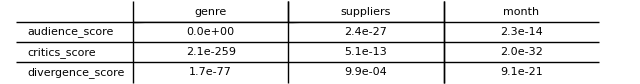
\includegraphics[width=1\textwidth]{imgs/var_p.png}
        \caption{p-values of a simple anova}
        \label{fig:variance_p}
    \end{figure}\\
    In figure \ref{fig:variance_p} we see that for all three we reject the zero hypothesis for each of these three scores.\\
    To further analyse between the means of which groups we see a significant difference in there mean, we use post hoc tests. The post hoc test uses a student t-test to test the differences between each pair of groups. The hypothesises for the student t test are as follows:
    \begin{enumerate}
        \item[H0:] The mean scores of the two groups are equal.
        \item[H1:] The mean scores of the two groups are different.
    \end{enumerate}
    For a significance level of 0.05 we get that the following percentages of the groups reject the zero hypothesis:\\
    \noindent
    \begin{figure}[h]
        \centering
        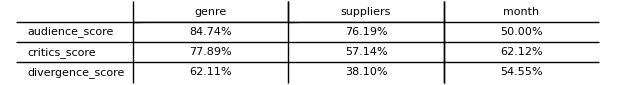
\includegraphics[width=1\textwidth]{imgs/prozent.png}
        \caption{percentage of the pairs of groups with significant deviation in mean messured by a student-t test}
        \label{fig:hypo_rejection}
    \end{figure}
    \FloatBarrier
    From this we can assume that genres, suppliers and release month offer use useful information for predicting our 3 target scores.

    \paragraph{Metric parameters}
    For metric parameters correlation is usually a good score to look at, when deciding whether a parameter contains useful information for our prediction or not. We used the pearsonr test, that has zero correlation as its zero hypothesis and a no-zero correlation as its alternative hypothesis. We got the following p-values:\\
    \noindent
    \begin{figure}[h]
        \centering
        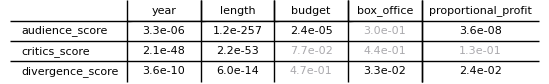
\includegraphics[width=0.94\textwidth]{imgs/metric_p.png}
        \caption{p-values of the pearsonr test}
        \label{fig:hypo_rejection}
    \end{figure}\\
    For year and film-length we reject the zero hypothesis for all 3 target scores. For the other parameter we only have enough evidence to reject the zero hypothesis for some of them. Since all of the parameters have a significant correlation to at least some of the target scores, we will include them in out training.
    
    
\subsection{Regression}
    As stated in the abstract, our goal was to predict the critics' score, the audience's score or the difference between the former (i.e. divergence).
    We used several different methods to transform our input parameters with significance to one of the three possible targets. All of the tested methods resulted in a bad fit.
    \paragraph{LinearRegression}
    We tried fitting the data with a simple linear regression model from the sklearn library. This generally resulted in the model predicting the mean of the targets for the training samples, whereas the Audience Model was the only one which could apply this to the test samples as well. Both Divergence and especially the Critics Model performed conclusively worse (\ref{tab:lin_regression}).
    \begin{table}[h]
        \centering
        \begin{tabular}{c||c|c|c|c}
             & Training score & Test score & Training MAE & Test MAE \\
            \hline
            Critics Model       & 0.057 & -945.89   & 22.83     & 39.68 \\
            \hline
            Audience Model      & 0.08  & 0.077     & 17.15     & 17.18 \\
            \hline
            Divergence Model    & 0.01  & -6.88     & 16.39     & 17.25
        \end{tabular}
        \caption{Linear Regression Scores and Mean Absolute Errors (MAE)}
        \label{tab:lin_regression}
    \end{table}

    \paragraph{CatBoost}
    CatBoost works on the theory of decision trees. It uses many weak models sequentially, to create a strong model. To achieve our target we used the Regressor (\texttt{CatBoostRegressor}) model from the CatBoost library.
    We see that the model suffers from overfitting (\ref{fig:mae_errors}). We tried to combat this be introducing L2-Regularizers, randomness in the choices on the decision-tree of CatBoost and adjusting the learning rate. Neither of them helped. 
    
    \paragraph{Neural Networks with PyTorch}
    Using PyTorch we created a model with three Hidden Layers (hidden width = 2 times input width) using Tanh, Leaky ReLU and ReLU as activation functions. It was not possible to use a higher Batch size since then our model would only generalize to predict the mean (similiar to linear Regression) thus the results depicted in (\ref{fig:mae_errors}) are created not using batches at all. But similarly to the CatBoost Regressor, only with slightly higher mean errors and less iterations, we achieve overfitting of the training samples and slight reduction in the test error. 
    
    \paragraph{Conclusion}
    We conclude that probably our parameters are not strong enough to predict either the score or the divergence. Our relatively low quantity of data (8000 training samples) is most likely too sparse for our objective and thus the algorithm only overfits without any significant generalization. But we could also observe that the predictions for the audience's score were more accurate, indicating that the audience score is possibly most influenced by the parameters we chose. There are more parameters such as production company, gender ratio of cast and producers that could be included already in our gathered data. Many more can be found by scraping more sources of data. The number of samples is way harder to increase, because the number of films released with scores on rotten tomatoes is limited.
    % Uns fehlen noch Angaben zum Mean und Varianz der Targets (i.e. Divergence MAE ist niedriger, aber varianz wird auch generell niedriger sein). Ok wenn du meinst wir brauchen das, sollte das wahrscheinlich zu analyse direkt??? Probably, aber ich denke es wäre nicht falsch die iwo stehen zu haben, damit besser nachvollziehbar ist, wie schwer die Daten zum erlernen sind OK
    % Ok die Varianz von Divergence ist nicht wirklich niedriger, bloß der Mean
    \begin{figure}[tb]
        \centering
        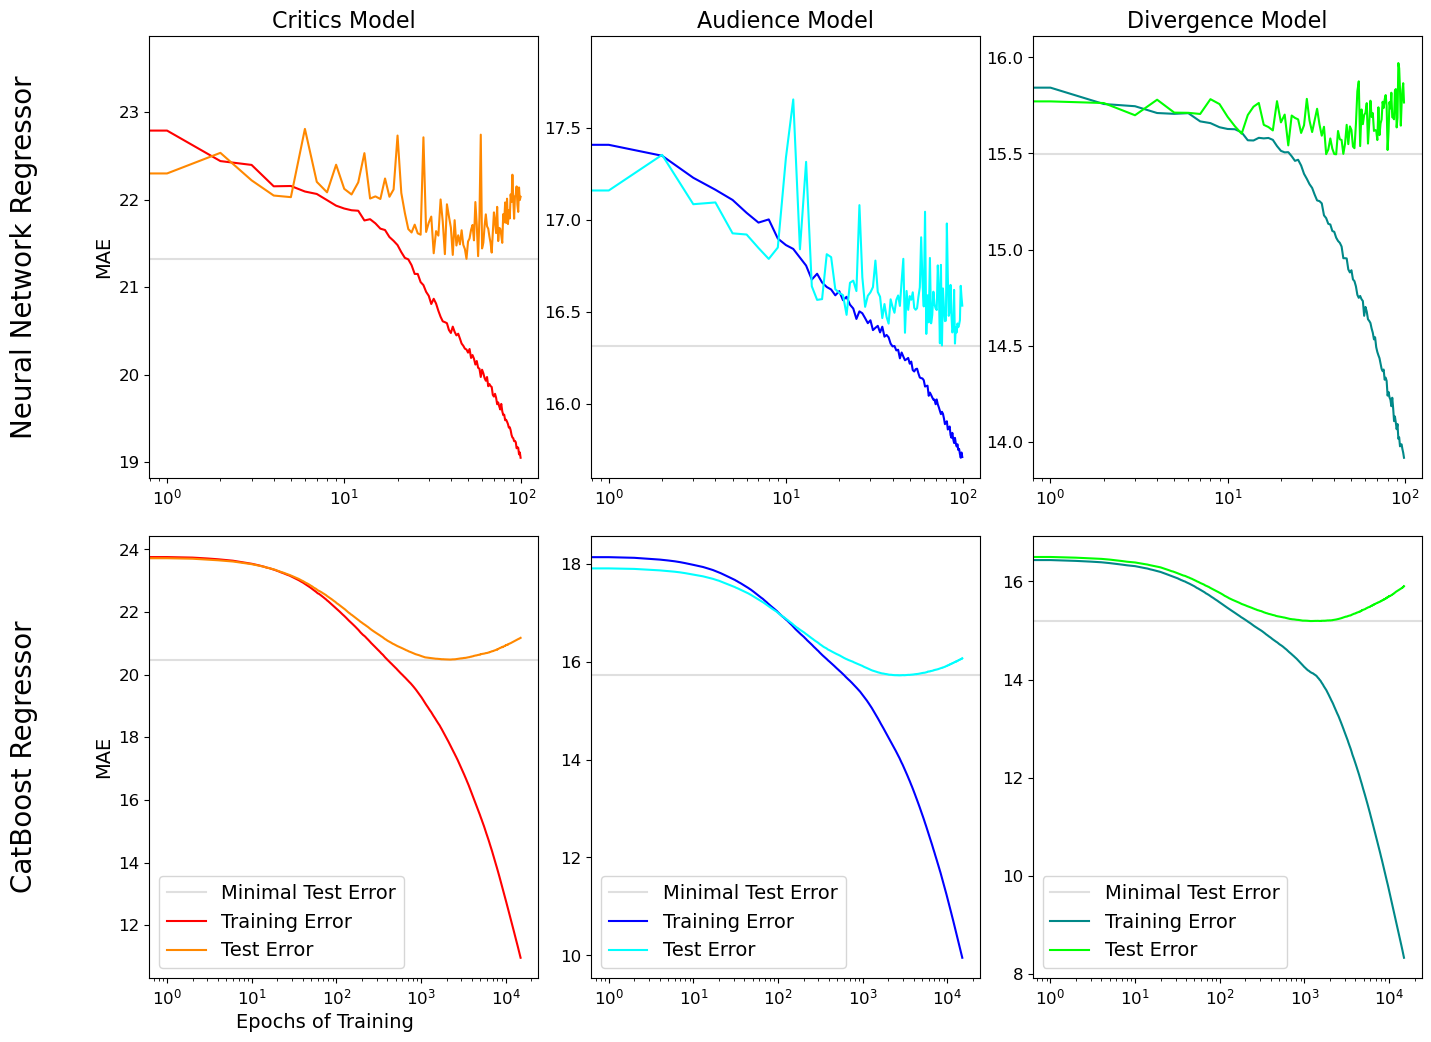
\includegraphics[width=1\textwidth]{imgs/regression_errors.png}
        \caption{Mean Absolute Errors during training of Neural Network- and CatBoost Regressors}
        \label{fig:mae_errors}
    \end{figure}

\bibliographystyle{abbrv}
\bibliography{sources}

\end{document}